\documentclass[12pt]{article}
% Must be compiled by XeLaTeX
\def\CNBtitle{Návod\ k\ použití\ třidy\ cnbwp}
\usepackage{cnbwp-manual}
\setdefaultlanguage{czech}
\title{Návod k použití třídy \fn{cnbwp} pro psaní Working~Papers~ČNB}
\author{Zdeněk Wagner}\date{verze 2013.12}
\def\?li{\discretionary{-}{-}{-}li}
\begin{document}
\maketitle

\begin{abstract}\noindent
Tento návod vysvětluje způsob psaní Working Papers České národní banky s použítím typografického
systému \LaTeX. Úvodní kapitoly se věnují popisu třídy \fn{cnbwp}, jež byla pro tyto účely
vytvořena. Samostatná kapitola popisuje způsob přípravy seznamu literatury. V následujících
kapitolách jsou uvedeny rady pro tvorbu a vkládání obrázků a tabulek. Kapitola~\ref{odevzdani}
obsahuje doporučení, v jaké podobě je nutné dokument odevzdat, kapitola~\ref{korektury} je vhodná
pro jazykové korektory. Jména maker, balíčků, souborů a programů, o nichž se v tomto návodu píše,
jsou setříděna v \hyperref[index]{rejstříku}. Součástí návodu jsou i vzorové soubory, jejichž výčet
najdete v kapitole~\ref{vzor}.
Třída s návodem i se vzorovými soubory byly vypracovány pro Českou národní banku.
\end{abstract}

\tableofcontents

\section{Typografické konvence}\label{typokon}
V tomto dokumentu bude užíváno několik typů písma se speciálním významem. Text tištěný
\texttt{neproporcionálním písmem} bude určen pro výpisy částí kódu tak, jak musí být uvedeny ve
zdrojovém souboru v \LaTeX{}u. Může se objevit i přímo v textu při popisu nějakého makra. V textu
se tedy může vyskytnout \cmd{usepackage} apod. Jména parametrů a jiných proměnných objektů budou
zapisována \textit{kurzívou}. V kapitole popisující způsob vytváření seznamu literatury budeme
používat zápis \bibi, kde \textit{typ} bude nahrazovat část jména makra. Budou tím obecně myšlena
makra \cmd{bookItem}, \cmd{miscItem} a další.

Pro zápis jmen souborů, balíčků a tříd bude použit \fn{bezpatkový font}. Příklad vidíte v názvu
dokumentu i v abstraktu. Výjimkou bude zápis URL, kde potřebujeme jisté speciální znaky. URL proto
budeme též tisknout \texttt{neproporcionálním písmem}, např.
\zwurl{ftp://ftp.cstug.cz/pub/tex/CTAN/}, ale zde nedojde k nedorozumění. Stejným způsobem budeme
zapisovat i plné názvy souborů s uvedenou cestou, např.
\zwurl{/usr/share/texmf-dist/tex/latex/cnb/cnbwp.cls}. Tyto dlouhé názvy lze rozdělit na více
řádků, přičemž není uveden rozdělovník.

Zdůrazněný text bude tištěn \textbf{tučným fontem}, protože kurzíva je již použita k jinému účelu.
Tučné písmo je užito i v nadpisech. V takové případě budou jména souborů, balíčků a tříd tištěna
\textbf{\fn{tučným bezpatkovým písmem}}.

\pozor Odstavec, začínající  velkým tučným červeným vykřičníkem, upozorňuje na velmi důležitou
informaci. Nerespektování uvedeného pokynu obvykle způsobí, že při zpracování dokumentu dojde k
závažné chybě, případně k chybě s exotickým hlášením, takže její příčinu nebude snadné najít.

\section{Instalace}\label{instalace}\index{instalace}
Veškerá makra pro psaní Working Papers České národní banky jsou implementována v třídě
\fn{cnbwp.cls}. Třída je distribuována v archivním souboru \fn{cnbwp.zip}. Soubor je v archivu
uložen s cestou odpovídající standardu TDS~(\TeX\ Directory Structure). Způsob instalace se
nepatrně liší v závislosti na konkrétní distribuci \TeX{}u.

\subsection{\MikTeX}\label{inst.miktex}
Soubor \fn{cnbwp.zip} rozbalíme do adresáře \url{X:\localtexmf}, kde \texttt{X:} označuje disk, na
němž je \MikTeX{} instalován (obvykle~\texttt{C:}). Poté otevřeme menu
\zwurl{Start/Programy/MikTeX/MikTeX Options}. Na kartě Roots si ověříme, že \url{X:\localtexmf} je
v seznamu prohledávaných adresářů. Pokud není, přidáme jej. Pak stiskneme tlačítko \texttt{Refresh
FNDB}. Úspěšnost instalace lze ověřit příkazem:

\begin{verbatim}
findtexmf cnbwp.cls
\end{verbatim}

\noindent Při úspěšné instalaci bude vypsána plná cesta k souboru \fn{cnbwp.cls}.

\pozor Adresář \url{X:\localtexmf} je určen pro místní soubory, které nejsou standardní součástí
\MikTeX u. Pokud přeinstalujete \MikTeX\ novou verzí, nebude tento adresář přepsán, takže o soubory
nepřijdete.

\subsection{\teTeX}\label{inst.tetex}
Tato distribuce je standardem v unixových systémech a je dostupná i pro OS/2 resp. eComStation.
Uvedeme si pouze instalaci v Linuxu. Instalace v OS/2 je obdobná. Liší se jen tím, že pro
oddělování adresářů je užito zpětné lomítko a musíme explicitně zadat označení disku, na nějž jsme
\teTeX\ nainstalovali.

Soubor \fn{cnbwp.zip} rozbalíme do adresáře \url{/usr/share/texmf-local}. Při instalaci v unixových
systémech je nutno dohlédnout na to, aby soubor
\url{/usr/share/texmf-local/tex/latex/cnb/cnbwp.cls} neměl DOSové konce řádků. Po rozbalení souboru
je obvykle nutné obnovit souborovou databázi příkazem \texttt{mktexlsr}.

Z této distribuce vychází i \TeXLive, proto vše, co bude popsáno v následující kapitole, platí i
pro \teTeX.

\subsection{\TeXLive}\label{inst.tl}
\TeXLive\ je oblíbenou multiplatformní distribucí \TeX{}u. Vychází ze stejných zdrojů jako
\hyperref[inst.tetex]{\teTeX}, instalace je tedy podobná. Adresář, do nějž rozbalíme
\fn{cnbwp.zip}, je většinou \url{/usr/local/texlive/texmf-local} v unixových systémech,
\url{X:\TeXLive\texmf-local} ve
Windows. \TeXLive\ však lze nainstalovat do libovolného adresáře a dokonce můžeme mít instalováno
několik verzí \TeXLive\ současně. Adresář, do nějž máme \fn{cnbwp.zip} rozbalit, zjistíme příkazem:

\begin{verbatim}
kpsewhich --expand-var=$TEXMFLOCAL
\end{verbatim}
\index{kpsewhich}

Adresářový strom \url{texmf-local} je sdílen všemi verzemi \TeXLive\ nainstalovaných na daném
počítači. Při instalaci novější verze \TeXLive\ budou soubory nalezeny automaticky.

\pozor Distribuce \TeXLive\ obvykle vyžaduje po přidání souborů spuštění programu
\texttt{mktexlsr}. V distribucích pro Windows pro tento účel existuje i položka v Menu \TeXLive.
Pokud programem \texttt{mktexlsr} neobnovíme databázi a před jménem adresáře s třídou \fn{cnbwp}
jsou uvedeny dva vykřičníky, \LaTeX\ nebude schopen třídu najít. Chceme\?li zjistit, zda \LaTeX\
třídu najde, použijeme příkaz:

\begin{verbatim}
kpsewhich cnbwp.cls -progname latex
\end{verbatim}

\noindent
Pokud je vše v pořádku, příkaz vypíše plnou cestu k souboru \fn{cnbwp.cls}.

\subsection{\emTeX}\label{inst.emtex}
Tato distribuce je zastaralá, Eberhard Mattes ji už neudržuje. Je vhodnější přejít na jinou
distribuci. Pokud přesto chcete používat \emTeX, rozbalte \fn{cnbwp.zip} do pomocného adresáře, v
adresáři \url{X:\emtex\texinput\latex2e} vytvořte podadresář \fn{cnbwp} a do něj zkopírujte soubory
\fn{cnbwp.cls} a \fn{cnbwpsizes.clo}.

\subsection{Scientific Word}\label{inst.sciword}
Návod je psán pro verzi 5.5. V této verzi rozbalte \fn{cnbwp.zip} do adresáře \url{X:\sw55\TCITeX},
v jiných verzích se pravděpodobně bude lišit jméno kořenového adresáře. Scientific Word nedodržuje
zcela přesně TDS, jména adresářů obsahují malá i velká písmena. Souborové systémy FAT a NTFS však
malá a velká písmena nerozlišují, takže by to nemělo způsobit žádný problém.

\subsection{Jiné distribuce}\label{inst.other}
Při instalaci třídy \fn{cnbwp} do jiných distribucí je nutno řídit se manuálem dodávaným s
příslušnou distribucí. Současné distribuce jsou založeny obvykle na \fn{web2c} a dodržují standard
TDS, proto lze postupovat obdobně jako při instalaci pro \hyperref[inst.tl]{\TeXLive, viz
kap.~\ref*{inst.tl}}.

\subsection{Zpracování dokumentů ze Scientific Wordu v~jiných
distribucích}\label{sciword.elsewhere}
Dokumenty vytvořené Scientific Wordem vyžadují určitá makra definobvaná v souborech v adresáři
\fn{SWmacros}. Tyto soubory jsou volně šiřitelné. Chcete\?li tedy dokument zpracovat v jiné
distribuci, zkopírujte celý adresář do \url{texmf-local/tex/latex} resp \url{localtexmf/tex/latex}
podle toho, jakou distribuci používáte.

\pozor Nezapomeňte, že v některých distribucích musíte po přidání souborů obnovit databázi buď
příkazem \texttt{mktexlsr}, nebo z menu.

\section{Testování instalace}\label{test.inst}
V mnoha distribucích lze správnost instalace otestovat příkazem \texttt{kpsewhich}, jak bylo uvedeno
v kapitole~\ref{inst.tl}. Můžeme tak ověřit, že \LaTeX\ dokáže najít třídu \fn{cnbwp} i makra z
adresáře \fn{SWmacros}. Nemáme\?li program \texttt{kpsewhich} ve své distribuci, stačí napsat
jednoduchý dokument:

\begin{verbatim}
\documentclass{cnbwp}
\begin{document}
Hello world.
\end{document}
\end{verbatim}

\noindent
Pokud \LaTeX\ při jeho zpracování nahlásí:

\begin{verbatim}
! LaTeX error: file `cnbwp.cls' not found
\end{verbatim}

\noindent
znamená to, že třída není instalována správně. V takovém případě si znovu ověřte správnost svého
postupu podle příslušné kapitoly.

\section{Struktura dokumentu}\label{struktura}
Working paper je běžným dokumentem psaným v \LaTeX{}u, skládá se tedy z obvyklých částí: z
preambule a z těla dokumentu. Do preambule patří vše, co je uvedeno před příkazem
\cmd{begin\{document\}}. Zvláštní částí těla dokumentu je seznam literatury. Tomu bude věnována
samostatná \hyperref[references]{kapitola~\ref*{references}}.

\subsection{Preambule}\label{preambule}\index{preambule}
Všechna základní makra jsou implementována v třídě \fn{cnbwp}. Každý dokument musí proto začínat
příkazem:

\begin{verbatim}
\documentclass{cnbwp}
\end{verbatim}

Příkaz \xx\cmd{documentclass} umožňuje zadávání parametrů v hranatých závorkách před jménem třídy.
Tak je tomu i v tomto případě. Třída \fn{cnbwp} je odvozena z třídy \fn{article} a přebírá všechny
parametry. Formát Working Papers je však pevně stanoven, proto parametry, jež mění
rozměry papíru, velikost písma a počet sloupců, jsou ignorovány.

V třídě \fn{cnbwp} lze použít několik nových parametrů. První z nich se týká číslování obrázků a
tabulek. Standardně jsou tabulky a obrázky číslovány nehierarchicky.
Způsob číslování lze volit. Nastavuje se těmito parametry:

\vb\noindent
\begin{tabular}{@{}Rl}
hierarchicalnumbering & hierarchické číslování \\
simplenumbering & jednoduché číslování
\end{tabular}\label{numbering}\index{hierarchicalnumbering}\index{simplenumbering}\vb

Pokud není žádný z těchto parametrů uveden, případně jsou uvedeny oba, bude se používat
jednoduché číslování.

Popisky obrázků a tabulek jsou standardně zarovnány na levý okraj. V některých dokumentech může
vypadat esteticky lépe, budou\?li popisy zarovnány na střed. Zarovnání pro celý dokument nastavíme
těmito parametry:

\vb\noindent
\begin{tabular}{@{}Rl}
standardcaptions & zarovnání popisků vlevo \\
centeredcaptions & zarovnání popisků na střed
\end{tabular}\label{captions}\index{standardcaptions}\index{centeredcaptions}\vb

Není\?li uveden žádný z těchto parametrů, nebo jsou uvedeny oba, budou popisky obrázků a tabulek
zarovnány vlevo.

Za určitých okolností je nutné některé popisky zarovnat jinak než ostatní popisy v dokumentu. Pro
tento účel slouží makra, která budou vysvětlena později v kapitole~\ref{body}.

Třída \fn{cnbwp} načítá implicitně balíčky, které jsou pro formátování Working Papers nezbytné. Jsou
to \xx\fn{ifpdf}, \xx\fn{mathptmx}, \xx\fn{fontenc} s parametrem T1, \xx\fn{babel} s parametry
czech a english, \xx\fn{natbib}, \xx\fn{url} a \xx\fn{keyval}. Parametry, uvedené v hranatých
závorkách v
příkazu \xx\cmd{documentclass}, jsou automaticky poslány všem těmto balíčkům, jakož i dalším
balíčkům,
které si zavedete sami později. Nejčastěji budete pravděpodobně specifikovat parametry pro balíček
\fn{natbib}. Budete\?li chtít změnit zápis citací z formátu autor-rok na číslované, použijete:

\begin{verbatim}
\documentclass[numbered]{cnbwp}
\end{verbatim}
\index{numbered}

Nyní můžete příkazem \xx\cmd{usepackage} načíst další balíčky potřebné pro
formátování svého
dokumentu. Lze uvést v jednou příkazu \cmd{usepackage} více balíčků oddělených čárkami, např.:

\begin{verbatim}
\usepackage{graphicx,amsmath,dcolumn}
\end{verbatim}

Makro \cmd{usepackage} též umožňuje uvádění parametrů v hranatých závorkách. Tyto parametry jsou
poslány pouze balíčkům uvedeným v daném příkaze. Pak ovšem nelze stejným příkazem načíst více
balíčků, protože by \LaTeX\ hlásil, že parametry nejsou v balíčku implementovány. Musíme použít
např.:

\begin{verbatim}
\usepackage{amsmath,dcolumn}
\usepackage[dvips]{graphicx}
\usepackage[figuresright]{rotating}
\end{verbatim}

Všem balíčkům budou poslány též parametry uvedené v příkazu \xx\cmd{documentclass}. Parametr
\texttt{draft} lze tedy specifikovat globálně:

\begin{verbatim}
\documentclass[draft]{cnbwp}
\usepackage{graphicx}
\end{verbatim}

\noindent
Můžeme jej však také použít jen s balíčkem \fn{graphicx}:

\begin{verbatim}
\documentclass{cnbwp}
\usepackage[draft]{graphicx}
\end{verbatim}

\noindent
V obou případech budou obrázky nahrazeny obdélníkovým rámečkem velikosti obrázku, v němž bude
vytištěno jméno souboru. V prvním případě budou navíc přetečené (over\-ful) boxy označeny na okraji
černými obdélníčky.

\pozor Balíček \xx\fn{hyperref} používá jinou definici makra \xx\cmd{url} než balíček \xx\fn{url}.
Tato
definice navíc způsobuje konflikty při zápisu odkazů. Třída \fn{cnbwp} proto zkopíruje definici
\cmd{url} z balíčku \fn{url} do pomocného makra \cmd{CNBurl} a po provedení \cmd{begin\{document\}}
je definice makra \cmd{url} obnovena tak, aby odpovídala balíčku \fn{url}. Chcete\?li používat makro
z balíčku \fn{hyperref}, uložte si jej po zavedení balíčku do makra s vhodným názvem, např. pomocí:

\begin{verbatim}
\let\MYurl\url
\end{verbatim}

\pozor
Nikdy neměňte definici makra \cmd{url}. Makra pro formátování seznamu literatury na jeho definici
spoléhají. Makro \cmd{url} může být použito v databázi citací zpracovávané \BibTeX em, takže v
dokumentu jej nemusíte přímo vidět. Při změně definice bude \LaTeX\ hlásit podivné chyby a
formátování části dokumentu se pravděpodobně zcela zhroutí.

\pozor
\LaTeX\ nevyžaduje používání oddělených jmenných souborů pro jednotlivé balíčky. Může se tedy stát,
že balíčky obsahují konfliktní definice, jež způsobí těžko předvídatelné chyby. Kromě výše zmíněné
kolize nelze současně s balíčkem \xx\fn{url} použít balíček \xx\fn{path}. Proto je vhodné začínat s
minimálním dokumentem a používat jen ty balíčky, jež jsou pro zpracování skutečně nezbytné. Kolize
je nutno hledat a odstraňovat metodou pokusu a omylu. Někdy pomůže i změna pořadí zavádění balíčků.

V závěru preambule je vhodné definovat vlastní makra potřebná v celém dokumentu. Pro definici maker
se zvlášť hodí příkaz \xx\cmd{DeclareRobustCommand}. Má stejnou syntaxi jako \xx\cmd{newcommand}.
Liší se jen tím, že definované makro je robustní. Při použití takto definovaného makra v příkazech
\cmd{section} a \cmd{subsection} nemusíte používat \xx\cmd{protect}.

\subsection{Titulní stránka}\label{titlepage}
Working Paper musí vždy začínat titulní stránkou, která se skládá z několika součástí. Jim budou
věnovány následující podkapitoly.

\subsubsection{Nadpis}\label{nadpis}
Nadpis je na pomezí preambule a těla dokumentu. Ve skutečnosti některá makra lze uvést již v
preambuli. Přesněji řečeno, makra, definující název, jména autorů a poděkování, lze zapsat kamkoliv mezi
\cmd{documentclass} a \cmd{maketitle}. Jejich uvedení na samém začátku souboru tedy může
být užitečné.

Název práce zadáváme jako argument makra \xx\cmd{title}. Název bude vytištěn později, až uvedeme
příkaz \xx\cmd{maketitle}, ale dostane se též do záhlaví:

\begin{verbatim}
\title{Fidlovačka aneb žádný hněv a žádná rvačka}
\end{verbatim}

Jména autorů zapisujeme pomocí makra \xx\cmd{author}, které vyžaduje dva parametry. V prvním
parametru je uvedeno plné jméno, v druhém parametru název instituce. Makro se uvede pro každého
autora samostatně např. takto:

\begin{verbatim}
\author{Kapitán Nemo}{Nautilus}
\author{Robinson Crusoe}{Pustý ostrov}
\end{verbatim}

Makro \xx\cmd{maketitle} doplní před jméno posledního autora spojku „and“ podle britských pravidel,
tj. čárka je uvedena pouze v případě, že práce má více než dva autory.
Jména autorů jsou též přenesena do záhlaví.

\subsubsection{Poděkování}\label{ack}
Poděkování je nepovinnou součástí Working Paper. Uvádíme jej v argumentu makra
\xx\cmd{acknowledge}.

Název práce bude vytištěn uvedením makra \xx\cmd{maketitle}. Toto makro se musí vyskytovat až za
\cmd{begin\{document\}}.

\subsubsection{Abstrakt}\label{abstrakt}
Práce musí obsahovat abstrakt ve dvou jazycích, nejprve anglicky, pak česky. Anglický abstrakt
uvádíme v prostředí \xx\texttt{abstract}, český v prostředí \xx\texttt{abstrakt}, tj. například takto:

\begin{verbatim}
\begin{abstract}
Place the abstract here.

The abstract may contain more than one paragraph. A blank line should be left
between the paragraphs. No blank line is needed at the end of the abstract.
\end{abstract}

\begin{abstrakt}
Zde uvedeme abstrakt práce.

Abstrakt může obsahovat více odstavců. Mezi odstavci ponecháme
prázdný řádek. Na konci abstraktu prázdný řádek být nemusí.
\end{abstrakt}
\end{verbatim}

V prostředí \xx\texttt{abstrakt} je automaticky aktivováno české dělení slov.

\subsubsection{JEL Codes}\label{jel}
JEL codes uvádíme v makru \xx\cmd{JEL}:

\begin{verbatim}
\JEL{E22, E23, E32, E52}
\end{verbatim}

\subsubsection{Klíčová slova}\label{kwd}
Klíčová slova jsou posledním elementem titulní stránky. Zadáváme je pomocí výše zmíněného makra
\xx\cmd{Keywords}:

\begin{verbatim}
\Keywords{Nautilus, moře, 2000 mil, velryba, malström}
\end{verbatim}

\subsection{Nontechnical Summary}\label{nontech}
Nontechnical Summary je text v rozsahu přibližně jedné stránky a v dokumentu je vytištěn na
samostatné straně. Zapisuje se, podobně jako abstrakt, do prostředí \xx\texttt{nontechsummary}:

\begin{verbatim}
\begin{nontechsummary}
V tomto prostředí zapisujeme Nontechnical Summary. Nadpis bude vyvořen
automaticky a nebude číslován.

Text se obvykle skládá z několika odstavců, jež jsou od sebe odděleny
prázdným řádkem.
\end{nontechsummary}
\end{verbatim}

\pozor
Makro \hyperref[kwd]{\xx\cmd{Keywords}} a prostředí \xx\texttt{nontechsummary} vynucují přechod na
novou
stránku. Pokud oba tyto elementy chybí a stránkový
zlom je vynucen ručně příkazem \cmd{newpage} nebo \cmd{clearpage}, nebude část dokumentu
naformátována správně.

\subsection{Makra pro tělo dokumentu}\label{body}
Tělo dokumentu je psáno stejně jako by byla použita běžná třída \fn{article}. Sekce tedy uvádíme
makrem \xx\cmd{section}, podsekce \xx\cmd{subsection}. Je implementován i příkaz
\xx\cmd{subsubsection}. S členěním až na \xx\cmd{paragraph} a \xx\cmd{subparagraph} nebylo při
návrhu počítáno, ale syntaktická chyba při použítí těchto maker nevznikne.

Popisky tabulek a obrázků zapisujeme do makra \xx\cmd{caption}. Popisek bude zarovnán podle toho,
jaký
parametr jsme uvedli v preambuli (viz \hyperref[captions]{str.~\pageref*{captions}}). Chceme\?li
jeden popisek zarovnat jinak, uvedeme explicitně \xx\cmd{standardcaption} pro zarovnání vlevo a
\xx\cmd{centeredcaption} pro zarovnání na střed. Způsob číslování vždy odpovídá parametrům uvedeným
v preambuli, jež jsou vysvětlena \hyperref[numbering]{na straně~\pageref*{numbering}}. V dokumentu
jej změnit nelze. Z typografického hlediska to ani nemá smysl.

V popisu tabulky či obrázku lze uvést poznámku pomocí makra \xx\cmd{Note} a informaci o zdroji
pomocí makra \xx\cmd{Source}. Tato makra se zpravidla uvádějí až pod makrem \xx\cmd{caption} podle
tohoto příkladu:

\begin{verbatim}
\Note{Value Added Tax (VAT), Excises (E), Personal Income Tax (PIT),
      Social Security Contributions (SSC), Inheritance Tax (IT),
      Corporate Income Tax (CIT), Other Age-Specific Revenues (OR).}
\Source{CNB}
\end{verbatim}

\section{Seznam literatury}\label{references}
Seznam literatury (bibliografii) lze zapisovat dvěma způsoby. V obou případech je k vlastnímu
formátování využit balíček \xx\fn{natbib}, jenž je automaticky načítán třídou \fn{cnbwp}.
Vzhled dokumentu tedy nezávisí na na tom, která metoda byla pro zápis seznamu literatury zvolena.

V kapitole~\ref{bibtex} bude stručně uveden způsob vytváření seznamu literatury při použití
\BibTeX{}u. V kapitole~\ref{makra} a jejích podkapitolách budou podrobně vysvětlena makra vytvořená
pro Working Papers České národní banky.

\subsection{Zápis pomocí \BibTeX{}u}\label{bibtex}\index{BibTeX@\BibTeX}
Použití \BibTeX{}u je popsáno v dokumentu Orena Patashnika \uv{\BibTeX ing}, jenž je součástí
běžných distribucí \TeX{}u. Využijeme stylu \xx\fn{abbrvcnb} odvozeného z bibliografických stylů balíčku
\xx\fn{natbib}. Předpokládejme, že bibliografickou databázi máme uloženu v souboru
\fn{odkazy.bib}. V \LaTeX ovém dokumentu pak uvedeme:

\begin{verbatim}
\bibliographystyle{abbrvcnb}
\bibliography{odkazy}
\end{verbatim}
\index{abbrvnat}\index{bibliography@\cmd {bibliography}}\index{bibliographystyle@\cmd
{bibliographystyle}}

\noindent
Po zpracování dokumentu \LaTeX{}em spustíme \BibTeX:

\begin{verbatim}
bibtex dokument
\end{verbatim}

\noindent
(Místo slova \textit{dokument} doplňte název souboru, zde jsme předpokládali, že dokument je uložen
v souboru \fn{dokument.tex}.) Pak je nutno zpracovat dokument dvakrát \LaTeX{}em. Výjimečně je
nutný ještě třetí průchod, pokud po doplnění odkazů do textu došlo ke stránkovému posunu.

URL dokumentů jsou většinou dlouhé řetězce, v nichž nefunguje automatické dělení slov, případně se
slova dělí na nevhodných místech a může dojít ke zmatení. Problém je řešen v souladu se standardy
pro zápis URL\index{URL} v balíčku \xx\fn{url}, který je též implicitně načítán třídou \fn{cnbwp}.
URL se obvykle vyskytuje v položce \textit{note}\index{note}. Tato položka by tedy měla být psána
způsobem:

\begin{verbatim}
note = "\url{ftp://ftp.cstug.cz/pub/tex/CTAN/}",
\end{verbatim}
\index{url@\cmd  {url}}

\subsection{Zápis pomocí speciálních maker}\label{makra}
Seznam literatury můžeme psát speciálními makry přímo v \LaTeX ovém souboru v prostředí
\xx\texttt{thebibliography}. Toto prostředí má jeden povinný parametr, z nějž se určuje šířka
potřebná
pro pořadové číslo. \BibTeX{} do tohoto parametru zapíše počet citací. Lze však uvést jakýkoliv
text vhodné šířky, například \texttt{XX}, jak je použito v příkladu (viz
\hyperref[priloha]{Příloha}). Jednotlivé citace jsou zapisovány ve tvaru:

\medskip\noindent
\bibi\texttt{[}\textit{text citace}\texttt{]}\texttt{\{}\textit{návěští}\texttt{\}}%
\texttt{\{}\textit{obsah citace}\texttt{\}}

\medskip\noindent
Místo slova \textit{typ} musíme uvést odpovídající typ citované práce. Použijeme identifikátor
odvozený ze standardních typů definovaných v \BibTeX{}u. Jejich seznam a popis bude uveden v
\hyperref[typy]{kapitole~\ref*{typy}}.

První dva parametry (nepovinný a povinný) mají stejný význam jako u makra \xx\cmd{bibitem}. Povinný
parametr \textit{návěští} je využíván při citování v textu v makru \xx\cmd{cite}, nepovinný
parametr
\textit{text citace} obsahuje údaj, který je v místě citace zapsán v textu. Tento parametr má
obecně tvar:

\medskip\noindent
\texttt{[}\textit{krátký text}\texttt{(}\textit{rok}\texttt{)}\textit{dlouhý text}\texttt{]}

\medskip
Balíček \fn{natbib} dokáže volit mezi uvedením krátkého a dlouhého textu. Pokud má citovaná
práce pouze jednoho autora, \textit{dlouhý text} se neuvádí. Celý parametr pak můžeme zapsat ve
tvaru:

\begin{verbatim}
[Pytlík(1984)]
\end{verbatim}

Obě varianty se uvádějí u prací s více autory. Chceme\?li například citovat knihu vydanou v roce
1984, jejímiž autory jsou Brouk Pytlík, Ferda Mravenec a Bába Krtonožka, zapíšeme parametr ve
tvaru:

\begin{verbatim}
[Pytlík et.~al.(1984)Pytlík, Mravenec a Krtonožka]
\end{verbatim}

\pozor
Při zpracování \BibTeX em jsou informace do makra \bibi\ vytvářeny automaticky. Pokud zadáváme
informace ručně, musíme správně doplnit parametr v hranatých závorkách. Informace v kulatých
závorkách tedy musí být identická s hodnotou pole \;year , jak je uvedeno mimo jiné v prvních dvou
položkách v příkladu v příloze~\ref{priloha}. \BibTeX\ seřadí citace abecedně, při přímém zápisu
musí citace správně seřadit autor.

Při volbě formátu textu citace vycházíme z požadavků, jak má výsledný text vypadat. Pokud
nepožadujeme dlouhou variantu odkazů, nemusíme ji v makru \bibi\ uvádět.

Balíček \xx\fn{natbib} nutně vyžaduje kulaté závorky v nepovinném parametru. Pokud není znám rok
zveřejnění citované práce, musíme uvést alespoň prázdné závorky~\texttt{()}.

V parametru \textit{obsah citace} zadáváme odkaz na citovanou práci. Formát parametru bude popsán v
\hyperref[obsah]{kapitole~\ref*{obsah}}.

\subsubsection{Typy citovaných prací}\label{typy}
Makra použitá pro citace prací vycházejí ze standardních typů definovaných v \BibTeX{}u. Zde
uvedeme jejich výčet a stručný popis včetně seznamu povinných a nepovinných položek. Význam položek
a způsob jejich zápisu bude vysvětlen v \hyperref[obsah]{následující kapitole}.

\begin{description}
\item[\xx\cmd{articleItem}] článek v časopisu. Povinné položky: \;author , \;title , \;journal ,
\;year . Nepovinné položky: \;volume , \;number , \;pages , \;month , \;note .

\item[\xx\cmd{bookItem}] kniha s uvedeným vydavatelem. Povinné položky: \;author \ nebo \;editor ,
\;title , \;publisher , \;year . Nepovinné položky: \;volume \ nebo \;number , \;series , \;address
, \;edition , \;month , \;note .

\item[\xx\cmd{bookletItem}] vytištěná a svázaná publikace bez uvedeného nakladatele a instituce.
Povinná položka: \;title . Nepovinné položky: \;author , \;howpublished , \;address , \;edition ,
\;month , \;year , \;note .

\item[\xx\cmd{conferenceItem}] viz \xx\cmd{inproceedingsItem}.

\item[\xx\cmd{inbookItem}] část knihy, obvykle kapitola nebo rozmezí stránek. Povinné položky:
\;author \ nebo \;editor , \;title , \;chapter \ a/nebo \;pages , \;publisher , \;year . Nepovinné
položky: \;volume \ nebo \;number , \;series , \;type , \;address , \;edition , \;month , \;note .
Význam položky \;type \ bude vysvětlen \hyperref[type]{na straně~\pageref*{type}}.

\item[\xx\cmd{incollectionItem}] část knihy mající vlastní název. Povinné položky: \;author ,
\;title
, \;booktitle , \;publisher , \;year . Nepovinné položky: \;editor , \;volume \ nebo \;number ,
\;series , \;type , \;chapter , \;pages , \;address , \;edition , \;month , \;note .
Položka \;type \ má stejný význam jako u předchozího typu citace a je vysvětlena \hyperref[type]{na
straně~\pageref*{type}}.

\item[\xx\cmd{inproceedingsItem}] článek ve sborníku konference. Povinné položky: \;author ,
\;title ,
\;booktitle , \;year . Nepovinné položky: \;editor , \;volume \ nebo \;number , \;series , \;pages ,
\;address , \;edition , \;month , \;organization , \;publisher , \;note .

\item[\xx\cmd{manualItem}] technická dokumentace. Povinná položka: \;title . Nepovinné položky:
\;author , \;organization , \;address , \;edition , \;month , \;year , \;note .

\item[\xx\cmd{mastersthesisItem}] diplomová práce. Povinné položky: \;author , \;title , \;school ,
\;year . Nepovinné položky: \;type , \;address , \;month , \;note .

\item[\xx\cmd{miscItem}] jiný typ užívaný v případě, že se nic jiného nehodí. Má pouze nepovinné
položky \;author , \;title , \;howpublished , \;month , \;year , \;note .

\item[\xx\cmd{phdthesisItem}] disertační práce. Povinné položky: \;author , \;title , \;school ,
\;year . Nepovinné položky: \;type , \;address , \;month , \;note .

\item[\xx\cmd{proceedingsItem}] sborník konference. Povinné položky: \;title , \;year . Nepovinné
položky: \;editor , \;volume \ nebo \;number , \;series , \;address , \;month , \;organization ,
\;publisher , \;note .

\item[\xx\cmd{techreportItem}] zpráva publikovaná školou nebo jinou institucí obvykle v číslované
sérii. Povinné položky: \;author , \;title , \;institution , \;year . Nepovinné položky: \;type ,
\;number , \;address , \;month , \;note .

\item[\xx\cmd{unpublishedItem}] dokument mající autora a název, avšak formálně nepublikovaný.
Povinné položky: \;author , \;title , \;note . Nepovinné položky: \;month , \;year .

\end{description}


\subsubsection{Specifikace položek}\label{obsah}
V posledním parametru maker \bibi\ je zapsán obsah jednotlivých položek citované práce. Položky se
uvádějí ve tvaru:

\begin{verbatim}
{jméno1 = hodnota1, jméno2 = hodnota2, jméno3 = hodnota3}
\end{verbatim}

\noindent
Mezery okolo znaků rovnítek a čárek, oddělujících jednotlivé položky, jsou ignorovány.
Ignorují
se též prázdné položky. Lze tedy napsat více čárek za sebou, čárku před první položkou a za
poslední
položkou. Všude, kde je povolena mezera, smíme též ukončit řádek. Kromě toho \TeX{} ignoruje
všechny mezery na počátku řádku. Seznam literatury proto můžeme zapisovat přehledně podobným
stylem, jaký je použit v \hyperref[priloha]{příloze}.

Položky se vzájemně oddělují čárkami. Pokud má být uvedena čárka v hodnotě položky, musíme celou
hodnotu uzavřít do složených závorek. Tento případ se bude nejčastěji vyskytovat při citaci prací s
více autory. Má\?li publikace pouze dva autory, jejichž jména jsou spojena spojkou \textit{a} (v
anglických pracích spojkou \textit{and}), budeme psát

\begin{verbatim}
author = Ferda Mravenec a Brouk Pytlík, ...
\end{verbatim}

\noindent
Zde čárka ukončuje položku. Máme\?li více autorů, musíme jejich jména uzavřít do závorek takto:

\begin{verbatim}
author = {Ferda Mravenec, Brouk Pytlík a Bába Krtonožka}, ...
\end{verbatim}

\noindent
První čárka (uvnitř závorek) je součástí seznamu autorů, druhá čárka ukončuje položku. V
anglických pracích uvádíme čárku před \textit{and} v případě, kdy citace má více než dna
autory.

\pozor Zapomenutá
čárka nebo vynechané závorky okolo hodnoty obsahující čárku mají za následek chybové hlášení o
neznámé položce s podivným jménem. Někdy se kvůli chybám tohoto typu může dokonce ztratit velká
část seznamu literatury i následujících částí dokumentu.

V databázových souborech určených pro zpracování \BibTeX{}em často používáme složené závorky, jimiž
zabraňujeme konverzi na malá či velká písmena. \LaTeX\ žádné konverze neprovádí, proto závorky
nepotřebujeme. Můžeme však použít různá makra, např. \xx\cmd{mbox} pro zabránění nevhodnému dělení,
\xx\cmd{-} k určení vhodného místa dělení slova, a dokonce si můžeme přímo uvnitř prostředi
\xx\texttt{thebibliography} definovat vlastní makra, jež budou v ostatních částech dokumentu
neznámá (nebo definovaná jinak).

Položky mohou být zapsány v libovolném pořadí, lze však použít pouze následující:

\begin{description}
\xitem[address] adresa nakladatele nebo instituce (např. školy u diplomových a disertačních prací)
\xitem[author] jména autorů v tom formátu, jak mají být uvedena, na rozdíl od \BibTeX{}u nedochází
k žádnému přeformátování (křestní jméno nebude zkráceno na iniciálu apod.).
\xitem[booktitle] název knihy, jejíž část je citována.
\xitem[chapter] číslo kapitoly.
\xitem[edition] vydání, mělo by to být pořadové číslo, které může být zadáno i slovně, např.
\textit{Second}.
\xitem[editor] jména editorů, zapisují se ve stejném formátu jako jména autorů.
\xitem[howpublished] způsob, jak byla zveřejněna práce neobvyklého typu.
\xitem[institution] instituce, která sponzorovala technickou zprávu (\cmd{techreportItem}).
\xitem[journal] jméno časopisu, resp. jeho zkratka.
\xitem[month] měsíc zveřejnění práce, v této položce lze uvést i den.
\xitem[note] vysvětlující poznámka. Tato položka je sice uvedena v příkladech v
\hyperref[priloha]{příloze}, ale v praxi ji budete užívat jen zřídka. Slouží k uvedení
URL\index{URL} prací
zveřejněných na Internetu, přičemž pro automatické a správné dělení dlouhých URL na více řádků se
používá balíček \xx\fn{url} načítaný třídou \fn{cnbwp}. URL tedy budete zadávat ve tvaru:

\begin{verbatim}
note = \url{ftp://ftp.cstug.cz/pub/tex/CTAN/}, ...
\end{verbatim}

\xitem[number] číslo časopisu, technické zprávy nebo práce vydávané v sérii.
\xitem[organization] organizace, která pořádala konferenci, nebo vydala manuál.
\xitem[pages] rozmezí stran.
\xitem[publisher] jméno vydavatele.
\xitem[school] škola, kde byla obhájena diplomová nebo disertační práce.
\xitem[series] jméno série (edice) knih.
\xitem[title] název práce.
\xitem[type] typ práce\label{type}, např. \textit{Research Note}. V citacích \xx\cmd{inbookItem} a
\xx\cmd{incollectionItem} specifikuje text odpovídající položce \;chapter \index{chapter}. Standardně
se doplní \texttt{chapter}, ale můžete zadat např. \texttt{section} nebo \texttt{kapitola}.
\xitem[volume] svazek časopisu nebo vícesvazkové knihy.
\xitem[year] rok vydání, u nepublikovaných prací rok napsání.
\end{description}

Členění na položky nemusí být dodržováno zcela striktně. Můžeme informace oddělit do samostatných
položek:

\begin{verbatim}
publisher = John Wiley \& Sons, address = New York, ...
\end{verbatim}

Seznam literatury, zapsaný přímo v \LaTeX ovém dokumentu, zřejmě nebude sloužit pro další strojové
zpracování. Může být proto účelné spojení obou informací do jedné položky:

\begin{verbatim}
publisher = {John Wiley \& Sons, New York}, ...
\end{verbatim}

\noindent Zde jsme museli použít závorky, protože spojená informace obsahuje čárku.

Makra automaticky doplňují tečky nebo čárky za jednotlivé položky, ale pouze v případě, že text
nekončí interpunkčním znaménkem. Mějme název zapsaný:

\begin{verbatim}
title = Can we spend less money for more music?, ...
\end{verbatim}

\noindent V tomto případě nebude interpunkční znaménko doplněno, a to ani v případě, kdyby celý
název byl uzavřen ve složených závorkách.

\subsection{Jak zvolit typ citované práce}
Typ citované práce musíme zvolit jak při zápisu do databáze pro \BibTeX, tak při použití maker
\bibi. Názvy typů jsou intuitivní a správná volba by měla být snadná. Ve sporných případech pomůže,
když si uvědomíme, které položky jsou povinné a které nepovinné. Zvolíme takový typ, jehož
struktura odpovídá účelu.

Některé položky jsou zdánlivě nadbytečné, např. diplomové (\xx\cmd{mastersthesisItem}) a disertační
(\xx\cmd{phdthesisItem})\footnote{V \BibTeX{}u \xx\texttt{@mastersthesis} a
\xx\texttt{@phdthesis}.} práce
jsou formátovány zcela stejně, liší se jen defaultní hodnota nepovinné položky \;type . Chceme\?li
citovat obdobnou publikaci, např. habilitační práci, můžeme použít kterýkoliv typ a specifikujeme
nepovinnou položku:

\begin{verbatim}
type = Habilitační práce, ...
\end{verbatim}

Práce dostupné pouze z Internetu nejsou formálně publikovány. Používá se pro ně
\xx\cmd{unpublishedItem}, v \xx\BibTeX{}u \texttt{@unpublished}. URL práce se uvede v položce
\;note \index{note}, jak bylo uvedeno výše.

\subsection{Technická poznámka}
V příkazu \cmd{documentclass} lze uvádět nepovinné parametry v hranatých závorkách. Tyto parametry
jsou poslány jak třídě \fn{article}, z níž je třída \fn{cnbwp} odvozena, tak všem načítaným
balíčkům. Lze tedy specifikovat parametry pro balíček \xx\fn{natbib}. Například parametrem
\xx\texttt{numbered} změníme citace ve tvaru autor-rok na číslované.

\pozor
Poslední parametr maker \bibi\ je zpracován pomocí balíčku \xx\fn{keyval}. Z toho vyplývá, že
smíme používat výhradně deklarované položky. Nelze vytvořit neznámou položku pro přidání komentáře,
který se nemá tisknout. Takový pokus vede k chybě při zpracování dokumentu. Komentáře zapisujeme za
znak \textit{procento} jako v běžných \LaTeX ových textech.

Nepovinný parametr a první povinný parametr maker \bibi\ jsou beze změny předány makru
\xx\cmd{bibitem}.

V případě, že požadovanému účelu nevyhovuje žádný z typů uvedených v kapitole~\ref{typy}, lze
použít přímo makro \xx\cmd{bibitem} a vše naformátovat ručně.

\section{Vkládání obrázků a~tabulek do textu}\label{vkladani}
Obrázky a tabulky vkládáme do textu prostřednictvím plovoucích prostředí \xx\texttt{figure} a
\xx\texttt{table}. V hranatých závorkách uvádíme nepovinně parametr, kde má být plovoucí objekt
umístěn. Tyto parametry \LaTeX\ ovšem chápe pouze jako doporučení. Nelze\?li jim vyhovět, pokusí se
o umístění plovoucího objektu na samostatnou stránku. Není\?li ani to možné, umístí příslušný
plovoucí objekt a všechny následující na konec dokumentu resp. kapitoly (v případě knih). Je tedy
nutno povolit více možností, aby si \LaTeX\ mohl vybrat. Uvedení samotného specifikátoru
[h]\index{h@[h]} obvykle vede právě k tomu, že je plovoucí objekt odsunut na samostatnou stránku či
konec dokumentu. O vynucené umístění plovoucího objektu na konkrétní místo si povíme v
kapitole~\ref{vynucene}.

\pozor Zde je vhodné místo k vysvětlení rozdílu mezi makry \xx\cmd{newpage} a \xx\cmd{clearpage} či
\xx\cmd{cleardoublepage}. První dvě vynutí přechod na novou stránku, \cmd{cleardoublepage} na
lichou stránku\footnote{To platí pouze pro oboustranně tištěné dokumenty, které mají explicitně či
implicitně specifikován parametr \xx\texttt{twoside}. Třída \fn{cnbwp} jej deklaruje implicitně.}.
Makra \cmd{clearpage} a \cmd{cleardoublepage} navíc vytisknou všechny dosud neumístěné plovoucí
objekty uschované ve vyrovnávací paměti.

Algoritmus umisťování plovoucích objektů se řídí hodnotami několika registrů. Hodnoty jsou voleny
pro běžné dokumenty, ale pro technické zprávy s mnoha tabulkami a obrázky nemusí být vyhovující.
Registr \xx\cmd{topfraction} určuje maximální část stránky, kterou smí zabrat plovoucí objekt
nahoře, \xx\cmd{bottomfraction} analogicky vymezuje maximální podíl stránky pro plovoucí objekty
umístěné dole a \xx\cmd{textfraction} je minimální část stránky, již musí zabírat text. Registry se
mění příkazem \xx\cmd{renewcommand}, neboť se jedná o makra. V dokumentech s mnoha plovoucími
objekty je můžeme nastavit na extrémní hodnoty pomocí:

\begin{verbatim}
\renewcommand\topfraction{.99}
\renewcommand\bottomfraction{.99}
\renewcommand\textfraction{.01}
\end{verbatim}

Plovoucí stránka je vytvořena pouze tehdy, pokud plovoucí objekty zaujímají alespoň část
definovanou v rexistru \xx\cmd{floatpagefraction}. Tuto hodnotu obvykle není nutno měnit.

\LaTeX\ má ještě čítače, jimiž nastavujeme nejvyšší povolený počet plovoucích objektů. Čítač
\xx\texttt{topnumber} určuje maximální počet plovoucích objektů nahoře, \xx\texttt{bottomnumber}
dole a \xx\cmd{totalnumber} omezuje celkový počet všech plovoucích objektů na stránce. Obvykle je
nemusíte měnit, k modifikacím by bylo nuno přistoupit jen v případě, že by dokument obsahoval velký
počet velmi malých plovoucích objektů\footnote{Pak by ale stálo za úvahu jejich seskupení s
využitím balíčku \xx\fn{subfigure}.}. Hodnoty se nastavují příkazem \xx\cmd{setcounter}, například:

\begin{verbatim}
\setcounter{totalnumber}{17}
\end{verbatim}

\pozor Aktuální hodnoty registrů lze zjistit různými způsoby. Zde si předvedeme použití příkazů
\TeX{}u \xx\cmd{show} a \xx\cmd{showthe}. První z nich slouží k zobrazení definice makra. Použijeme
jej tedy ke zjištění hodnoty registru typu \textit{fraction}. Registr typu \textit{number} musíme
vypsat pomocí \cmd{showthe}. Následující dva řádky vypíší aktuální hodnoty registrů
\cmd{topfraction} a \cmd{topnumber}:

\begin{verbatim}
\show\topfraction
\showthe\value{topnumber}
\end{verbatim}

\noindent Na terminálu a v log-souboru (zde jsme vypustili prázdné řádky) pak najdeme výpis podobný
tomuto:

\begin{verbatim}
> \topfraction=\long macro:
->.7.
l.875 \show\topfraction

> 2.
<recently read> \c@topnumber
l.876 \showthe\value{topnumber}
\end{verbatim}

\noindent Zjistili jsme tedy, že \cmd{topfraction} = 0.7 a \texttt{topnumber} = 2. Tečky na konec
definic přidávají příkazy \cmd{show} a \cmd{showthe}.

\subsection{Vynucené umístění plovoucího objektu na konkrétní místo}\label{vynucene}
V některých případech se stává, že plovoucí objekt \textbf{musí} nezbyně být na jistém konkrétním
místě. Potřebujeme tedy \LaTeX{}u sdělit, že specifikátor nemyslíme jako doporučený, nýbrž jako
kategorický příkaz. K tomu slouží specifikátor [H]\index{H@[H]}. Původně byl implementován v
balíčku \xx\fn{here}, ale ten již není v běžných distribucích. Tento specifikátor je nyní
implementován v balíčku \xx\fn{float}.

\pozor Při použití specifikátoru [H] prostředí přestává být plovoucím. \LaTeX\ jej umístí na
požadované místo bez ohledu na to, zda se do zbývajícího prostoru na stránce vejde. Používejte
proto tento specifikátor až ve finální verzi dokumentu.

\section{Příprava obrázků}\label{obrazky}
Tato kapitola se bude věnovat práci s obrázky. Nejprve si vysvětlíme rozdíly mezi hlavními
grafickými formáty. Dále si popíšeme, jak načteme obrázky do dokumentu, a nakonec uvedeme několik
postupů, jak obrázky připravovat a jak opravit obrázky vytvořené špatně napsanými programy.

\subsection{Grafické formáty}\label{graform}
Obrázky podle formátu dělíme na dva základní typy: bitmapové a vektorové. Bitmapové obrázky
představují matici hodnot (rastr), přičemž každý prvek nese informaci o barvě zobrazeného bodu
nenulové
velikosti. Vektorové obrázky se liší tím, že jsou v nich křivky popsány matematickými rovnicemi a
ke každé křivce je přidána informace o tloušťce čáry, její barvě, případně o barvě, jíž má být
vyplněna ohraničená plocha. K převodu na rastr dochází až v okamžiku zobrazení na monitoru či
tisku.

Zdálo by se, že není velký rozdíl ve výsledku, protože vektorový obrázek se také musí vyrastrovat,
ale opak je pravdou. Zásadní rozdíl je v tom, že každé zobrazovací či tiskové zařízení má jiné
rozlišení, tj. jinou hustotu rastru. Vektorový obrázek se rastruje v okamžiku zobrazení, je tedy
rastrován na konkrétní rozlišení. Záleží též na velikosti a tvaru tiskových bodů. Podle toho se
určuje barva bodů, jež jsou matematicky na hranici mezi obarvenou a neobarvenou částí roviny.
Rasterizační algoritmus zobrazovacího zařízení je vypočte tak, aby křivky vypadaly hladce.

Při zobrazení bitmapového obrázku je nutno zachovat předepsanou velikost, přestože byl vytvořen pro
jiné rozlišení. Nezbývá tedy jiná možnost než body dopočítat interpolací. V bitmapovém obrázku již
nemáme informaci, zda bod ležel na nějaké křivce. Přestože ovladač příslušného zažízení zná
velikost a tvar tiskových bodů, nemá dost informací, aby je při rastrování mohl použít.

Příklad vektorového a bitmapového grafu je uveden na obrázku~\ref{vectbitfig}. Obrázek je jedním z
demonstračních příkladů dodávaných s programem gnuplot. Ze stejného zdroje byla vytvořena vektorová
i bitmapová podoba.

\begin{figure}[p]
{\centering
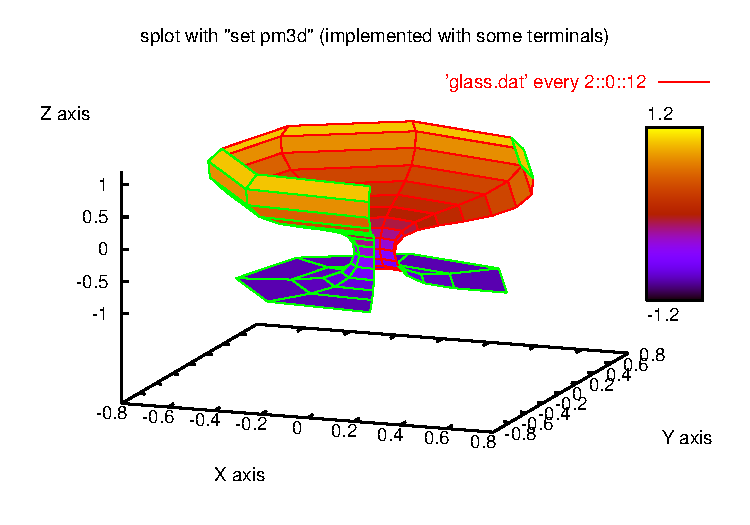
\includegraphics[width=.61\textwidth]{graph18.pdf}

\hrule \vskip 2dd

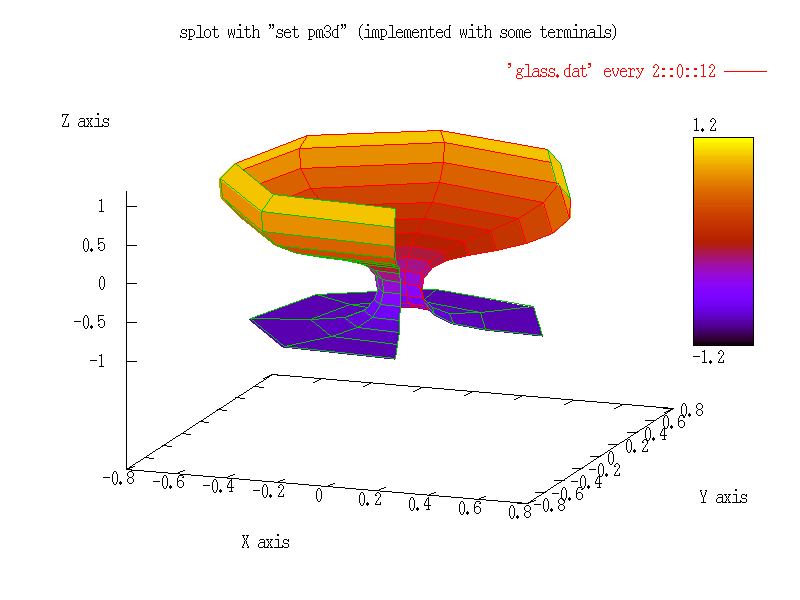
\includegraphics[width=.61\textwidth]{graph18.png}

\hrule \vskip 2dd

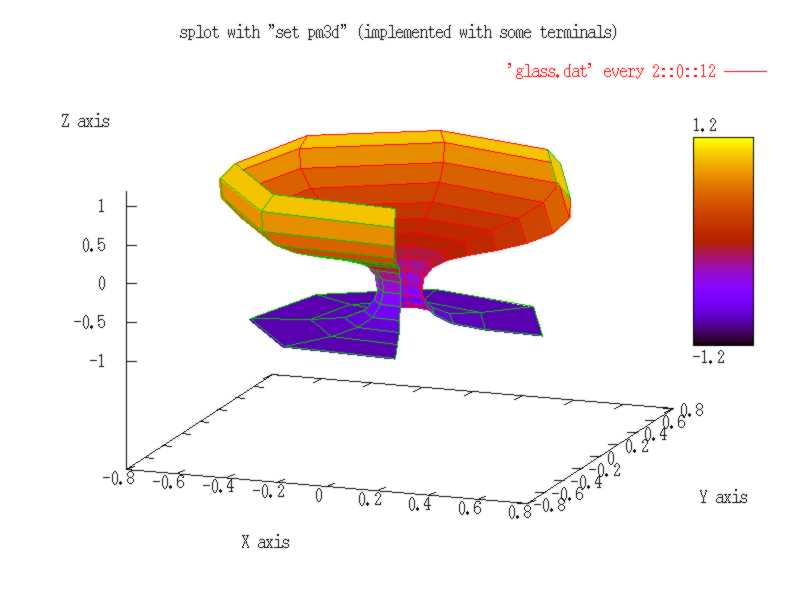
\includegraphics[width=.61\textwidth]{graph18.jpg}

}
\caption{Srovnání vektorového obrázku (nahoře) s~bitmapovým s~bezztrátovou kompresí (uprostřed)
a~ztrátovou kompresí JPEG (dole)}\label{vectbitfig}
\end{figure}

Horní obrázek je vektorový. Byl exportován jako EPS\index{EPS} (Encapsulated
Post\-Script\index{Encapsulated PostScript}) a převeden na PDF, aby mohl být načten pdf\TeX em nebo
\XeTeX em. Na
obrazovce mohou být křivky zubaté, protože rozlišení obrazovky je malé, ale po vytištění na
kvalitní tiskárně zuby zmizí.

Střední obrázek byl exportován ve formátu PNG\index{PNG} (Portable Network Graphics\index{Portable
Network Graphics}). Rozdíl v kvalitě zobrazení je zřejmý, zejména výrazné je zhoršení kvality
písma. Při určitém zvětšení mohou zcela zmizet osy. Osy zůstanou zubaté i po vytištění na tiskárně
s vysokým rozlišením, neboť, jak již bylo napsáno, ovladač příslušného zařízení neví, že body měly
ležet na jedné přímce, a pouze \uv{schody} přepočítá na jiné rozlišení.

Rastrová data zabírají příliš mnoho paměti. V obrázcích se však vyskytují opakované sekvence barev
a jednobarevné plochy. Data lze tedy uložit ekonomičtěji využitím nějakého kompresního algoritmu.
Kompresní algoritmy dělíme do dvou skupin, na bezztrátové a ztrátové. Bezztrátové algoritmy se
vyznačují tím, že lze dekompresí obnovit původní data. U ztrátových algoritmů to v principu nelze.

Formát PNG, použitý na středním obrázku, používá bezztrátový kompresní algoritmus. Spodní obrázek
byl uložen ve formátu využívajícím ztrátovou kompresi JPEG\index{JPEG}\footnote{Vyslovuje se
\textit{jay peg}.}. Tento algoritmus vyvinulo
konsorcium Joint Photographic Expert Group\index{Joint Photographic Expert Group} pro ukládání
barevných fotografií. Výzkumem bylo zjištěno, které obrazové elementy lidské oko nerozezná. Není
tedy na závadu, jsou\?li z fotografie odstraněny. Kvalita není zhoršena a výrazně se zmenší velikost
souboru. Kvalitu obrázku lze ovlivnit, ale i při nejvyšší kvalitě zobrazení (nejméně účiné
kompresi) je vždy komprese ztrátová. Formát se nazývá JFIF\index{JFIF} (JPEG File Interchange
Format\index{JPEG File Interchange Format}) a soubory mají nejčastěji příponu \xx\texttt{jpg}, méně
často \xx\texttt{jpeg}, \xx\texttt{jff} nebo \xx\texttt{jfif}.

Spodní obrázek byl vytvořen v nízkém rozlišení, vhodném pouze pro obrazovku, a uložen úmyslně s
nastavenou nízkou kvalitou, aby bylo na první pohled zřejmé, že při použití ztrátové komprese
dochází k rozmazání a k vytvoření barevných artefaktů, zejména v téměř jednobarevných plochách.

\pozor
Pamatujme si, že obrázky vždy vytváříme v takovém formátu, který nejlépe odpovídá jejich
charakteru. Grafy a diagramy jsou vždy matematické objekty, které lze popsat rovnicemi známými z
analytické geometrie. Komplikované křivky jsou přitom obvykle aproximovány Bézierovými křivkami.
Obrázky tedy vytvoříme ve vektorovém formátu. Bitmapové formáty používáme pouze pro obrázky, které
nemají matematickou reprezentaci. Přednost dáváme formátům s bezztrátovou kompresí. Grafické
formáty se ztrátovou kompresí používáme \textbf{výhradně na barevné fotografie a na nic jiného}!

Ohledně grafických formátů panuje mnoho nepravdivých pověr. Jednou z nich je domněnka, že formát
EPS\index{EPS} je vektorový. Je to pravda pouze částečná. Formát EPS je v zásadě Post\-Script s
jistými omezeními. Soubor může obsahovat jak vektorovou, tak bitmapovou grafiku, a to dokonce
jejich kombinaci. Při ukládání obrázku ve formátu EPS tedy záleží na tom, jakým programem jsme jej
vytvořili. Pokud byl obrázek nakreslen bitmapovým editorem, jakými jsou např.
Photoshop\index{Photoshop} nebo Gimp\index{Gimp}, bude i výsledný EPS bitmapový. Totéž platí o
formátu PDF\index{PDF}. Oba formáty povolují u bitmapových obrázků bezztrátovou i ztrátovou
kompresi.

Mnoho lidí se omylem domnívá, že není rozdílu mezi formáty PS\index{PS}
(Post\-Script\index{PostScript}) a EPS\index{EPS}. Bohužel se tímto velmi oblíbeným omylem nechali
svést i někteří autoři komerčních programů. EPS povoluje pouze podmnožinu jazyka Post\-Script a
vyžaduje nějaké informace navíc, aby programy dokázaly vložit obrázek do dokumentu. Některé
programy však vytvářejí postscriptové soubory, jež se jen tváří jako EPS. V některých případech to
nevadí, ale často takový obrázek vložit nelze, protože to způsobí podivné chyby (poškodí se
následující obrázek, ztratí se část textu, nebo i celý zbytek dokumentu). Expert někdy dokáže
takový soubor opravit, ale může to vyžadovat několikahodinové studium. Naštěstí existují nástroje,
které takovou nápravu zvládnou\label{poprava}. Zmíníme se o nich v kapitole~\ref{oprava}.

Další pověra se týká bitmapového formátu TIFF\index{TIFF} (Tagged Image File Format\index{Tagged
Image File Format}, soubory mají obvykle příponu \xx\texttt{tif}). Obvykle se tvrdí, že tento
formát používá bezztrátovou kompresi. Ve skutečnosti si však při ukládání můžeme kompresi zvolit.
Máme na výběr několik bezztrátových algoritmů, dokonce lze obrázek uložit zcela bez komprese, ale
můžeme též použít ztrátovou kompresi JPEG.

\subsection{Načtení obrázku do dokumentu}\label{incgraph}
V kapiole~\ref{vkladani} jsme se věnovali plovoucím prostředím a metodám, jak vložit plovoucí
objekt do textu. Nyní se zaměříme na to, jak do plovoucího prostředí načteme vlastní obrázek.

\TeX\ je program napsaný pro zpracování textu. Kromě primitivní grafiky tvořené vodorovnými a
svislými úsečkami a znaky ze speciálně připravených fontů nelze žádné obrázky přímo vytvářet.
Neexistuje ani příkaz pro vložení obrázku. \TeX\ má ovšem příkaz \xx\cmd{special}, který není vůbec
interpretován a jeho argument je pouze poslán výstupnímu zařízení. Záleží na příslušném ovladači,
jak s takovým povelem naloží. Mluvíme\?li o tom, jak se do \TeX ových či \LaTeX ových dokumentů
vkládají obrázky, máme vždy na mysli nějaký konkrétní ovladač zařízení.

Working Papers České národní banky jsou zveřejňovány ve formátu PDF\index{PDF}. Zaměříme se tedy na
dvě nejběžnější metody, jak získat PDF z textu psaného v \LaTeX u. První možností je konverze
souboru DVI na \xps\ programem \xx\fn{dvips}. Postscriptový soubor pak převedeme na PDF nějakým
programem (existují komerční i volně šiřitelné programy). Druhou možností je přímá tvorba
PDF\index{PDF} programem \xpdftex.

Při použití programu \fn{dvips} je optimálním grafickým formátem EPS\index{EPS}, a to jak pro
bitmapové, tak pro vektorové obrázky. Program \pdftex\ umí načíst přímo obrázky ve formátech
JFIF\index{JFIF} a PNG\index{PNG}, ale ty jsou bitmapové a budeme je používat jen zřídka. Vektorové
obrázky musíme připravit ve formátu PDF. Pro převod z EPS do PDF lze využít komerční Adobe
Distiller\index{Distiller}\index{Adobe Distiller}. Stejnou funkci však nabízí i program
\xx\fn{epstopdf}. Ten však vyžaduje \xgs\ a \xx\fn{perl}. Zmíněné programy jsou volně šiřitelné a
existují pro všechny operační systémy.

Obrázek lze načíst různými způsoby. Nejpohodlnějším je zřejmě využití balíčku \xx\fn{graphics}.
Makro \xx\cmd{includegraphics} má jeden povinný parametr, jímž je jméno souboru obsahujícího
obrázek. V nepovinném parametru v hranatých závorkách lze uvést řadu rozličných pokynů ve tvaru
\textit{klíč=hodnota}. Syntaxe je stejná jako u makra \bibi, jež bylo popsáno v
kapitole~\ref{obsah}, pouze místo složených závorek používáme závorky hranaté, neboť první
parametr je nepovinný. I zde jsou parametry zpracovány pomocí balíčku \xx\fn{keyval}.

Podrobný popis příkazu \cmd{includegraphics} najdete v souboru \xx\fn{grfguide.ps}, jenž je
součástí distribuce. Zde si popíšeme pouze několik základních parametrů:

\begin{description}
\xitem[scale] je poměr zmenšení či zvětšení. Zmenšení na polovinu dosáhneme zadáním
\texttt{scale=.5}.
\xitem[width] specifikujeme požadovanou šířku. Rozměr lze zadat v libovolných jednotkách, ale i
jako podíl jiných rozměrů. Požadujeme\?li šířku 75\,\% šířky textu, použijeme
\verb;width=.75\textwidth;.
\xitem[height] určuje výšku obrázku. Uvedeme\?li současně \texttt{height} i \texttt{width}, dojde k
distorzi obrázku. Použijeme\?li pouze jeden z těchto parametrů, druhý z nich se dopočte tak, aby
poměr stran zůstal zachován.
\xitem[clip]\label{clip} způsobí oříznutí na ohraničovací rámeček. Některé programy (např. Quatro)
vytvářejí
vadné EPS, jež vymažou své okolí. Pokud při vložení obrázku zmizí část textu nad ním nebo vedle
něho, vyzkoušejte použití parametru \texttt{clip} (bez uvedení rovnítka a hodnoty).
\xitem[page] používáme pouze při vkládání obrázku z vícestránkového souboru PDF\index{PDF}.
Zadáváme jím pořadové číslo stránky, kterou chceme vložit.
\end{description}

\subsection{Příprava vektorového obrázku}\label{makevectfig}
Připravujeme\?li vektorový obrázek, musíme především použít grafický editor nebo obdobný program,
který skutečně pracuje s vektorovou reprezentací. Obrázek pak musíme převést do formátu, který
lze do dokumentu načíst, tj. EPS nebo PDF. Výhodou je, pokud program umí soubor v tomto formátu
zapsat přímo. V opačném případě si musíme pomoci nějakou náhradní metodou.

V následujících podkapitolách si popíšeme několik běžných programů a ukážeme si úskalí, jež nás
mohou potkat.

\subsubsection{Gnuplot}\label{gnuplot}\index{gnuplot}
Gnuplot je flexibilní volně šiřitelný program pro kreslení matematických grafů. Je dostupný pro
všechny operační systémy. Byl jím vytvořen obrázek~\ref{vectbitfig}. Umožňuje výstup v mnoha
formátech včetně EPS\index{EPS}, nové verze i v PDF\index{PDF}.

Program nabízí bohaté možnosti ovlivňování barvy křivek i bodů a tvaru bodů. Tyto možnosti závisí
na zvoleném výstupním formátu, dokonce stejný typ křivky může být v různých výstupních formátech
zobrazen jinou barvou. Informaci získáte nejlépe pomocí příkazu \texttt{test}, jíž získáte
testovací obrazec představující všechny možnosti příslušného formátu. Chcete\?li zjistit, jaké
možnosti poskytuje výstup ve formátu EPS, použijte příkazy:

\begin{verbatim}
set term postscript eps color solid lw 2 18
set output "test.eps"
test
set output
quit
\end{verbatim}

\noindent
Testovací obrazec bude v souboru \fn{test.eps} v aktuálním adresáři.

\subsubsection{Corel Draw}\label{corel}\index{Corel Draw}
Corel Draw je komerční editor vektorových obrázků. Nabízí funkci exportu do formátu EPS. Nesmíme
však zapomenout, že Corel Draw obsahuje spoustu písem, jež nejsou dostupná na jíných počítačích.
Při exportu do EPS je proto musíme převést do křivek. Počínaje verzí~8 již tuto akci program
provede automaticky.

\subsubsection{Adobe Illustrator}\label{ai}\index{Illustrator}\index{Adobe Illustrator}
Adobe Illustrator je komerční vektorový editor, jehož nativní formát AI\index{AI} je založen na
\ps{}u. Otevřeme\?li soubor v běžném textovém editoru, na první pohled jej nerozeznáme od EPS. \ps\
je však programovací jazyk, jenž má s \TeX em jeden společný rys: umožňuje definici uživatelských
příkazů (operátorem \texttt{def}). Formát AI sice obsahuje postscriptové příkazy, ale pro jejich
interpretaci je nutno mít nadefinována makra, jež má Adobe Illustrator v sobě. Pokud vložíte do
jiného dokumentu přímo obrázek ve formátu AI, vše bude zdánlivě fungovat, ale jen do chvíle, kdy se
pokusíte dokument vytisknout. Na stránce, obsahující tento obrázek, interpret \ps{}u nahlásí chybu
typu \texttt{undefined}. Nezapomeňte proto uložit obrázek ve formátu EPS.

\subsection{Virtuální tiskárny}\label{virt}
Virtuální tiskárny představují náhradní řešení pro případ, že program nemá výstup do formátu EPS.
Metoda je ovšem použitelná pouze v případě, že používáme vektorový editor. Bitmapový grafický
editor i při použití virtuální tiskárny vytvoří bitmapový EPS či PDF.

\subsubsection{Tiskárny s~výstupem do \ps{}u}\label{virtps}
Na trhu jsou dostupné tiskárny s podporou \xps{}u. Pro tyto tiskárny existují ovladače, jež jsou
běžnou součástí instalačního CD operačního systému (Windows, Mac~OS, OS/2, eComStation). Některé
tiskárny podporují více komunikačních jazyků, jakými jsou PCL\index{PCL} a HPGL\index{HPGL}.
Použití takového ovladače ve funkci virtuální tiskárny není vhodné, neboť na začátku a na konci
vygenerovaného souboru jsou obvykle příkazy jazyka PJL\index{PJL} nebo obdobného, jimiž se zapíná a
vypíná interpret jazyka \xps. Takové příkazy nám pro další zpracování napáchají více škody než
užitku. Nejlepší jsou většinou tiskárny Apple Writer, případně speciální virtuální ovladače
získané z \url{http://www.adobe.com}. Chceme\?li vytvářet barevné obrázky ve formátu EPS\index{EPS},
musíme nainstalovat ovladač barevné tiskárny. Ovladač černobílé tiskárny totiž může převést barvy
na stupně šedi.

Chceme\?li nainstalovat virtuální tiskárnu ve Windows, je důležité z několika možností zvolit tu
nejlepší. Tiskárnu instalujeme jako lokální a nepřipojíme ji k žádnému fyzickému zařízení, nýbrž k
souboru. Pokud ovladač umožňuje nastavení funkcí, zapneme formát EPS, požadujeme konverzi fontů na
Type~1 a jejich vkládání do dokumentu. Při tisku \textbf{nesmíme zaškrtnout tisk do souboru}, ale
vyčkáme, až nás ovladač k zadání jména souboru sám vyzve.

\subsubsection{Tiskárny s~výstupem do PDF}\label{virtpdf}
Virtuální tiskárnu s výstupem do PDF\index{PDF} nabízí komerční Adobe
Acrobat\index{Acrobat}\index{Adobe Acrobat}. Existuje též řada sharewarových programů generujících
PDF, jež se nainstalují jako virtuální tiskárny. Všechny mají svůj vlastní instalační program. Opět
se snažíme, je\?li to možné, zapnout konverzi fontů na Type~1 a vkládání fontů do dokumentu.

\subsection{Oprava vadných souborů EPS a~PDF}\label{oprava}\index{EPS}\index{PDF}
V kapitole~\ref{poprava}, na straně~\pageref{poprava}, jsme se zmínili o tom, že obrázky v
souborech EPS a PDF mohou být poškozeny. Nyní si popíšeme, jak je lze opravit.

První častou chybou je nesprávný či nevhodný ohraničovací rámeček (BoundingBox\index{BoundingBox}).
Ohraničovací rámeček označuje rozměry obrázku v souboru EPS. Podle specifikace musí být veškerý
obrázek uvnitř rámečku, ale není řečeno, že musí být rámeček těsný. Pokud je ohraničovací rámeček
příliš velký, není to chyba, ale není to užitečné. Podle této informace totiž program vkládá
obrázek do dokumentu. Je\?li ohraničovací rámeček příliš velký, vynechá program okolo obrázku velké
volné místo. Nápravy nejlépe dosáhneme volně šiřitelným programem \xgs\ a jeho pohodlnou
nadstavbou \xgv. Potřebujeme oba programy, pro Linux exisuje řada různých nadstaveb (např.
\xx\fn{ggv} pro Gnome). Přepneme orientaci obrázku na Portrait a zvolíme funkci s nepřiliš vhodným
názvem \texttt{PS~to~EPS}. Funkce totiž nekonvertuje \ps\ na EPS, pouze vygeneruje těsný
ohraničovací rámeček se správnými rozměry. V naprosté většině případů funguje správně automatické
nastavení. Ruční nastavení využijeme v případech, kdy automat selže, nebo v případech, kdy se
chceme části obrázku zbavit a plánujeme použití parametru
\hyperref[clip]{\texttt{clip}}\index{clip} v makru \xx\cmd{includegraphics}.

\pozor \gv\ neumí zjistit potřebnou velikost papíru pro zobrazení obrázku ve formátu EPS. Navíc
některé programy, zejména virtuální tiskárny, nevloží obrázek do levého dolního rohu. Pokud vidíte
pouze prázdnou stránku, zkuste v menu Media zvolit větší velikost papíru.

Rozměry stránky v souboru PDF změníme pomocí plného Adobe Acrobatu\index{Acrobat}\index{Adobe
Acrobat}, jenž tuto funkci nabízí. Neznám volně šiřitelnou alternativu.

Horší situace nastane, jestliže se soubor pouze tváří jako EPS. Nejjednodušší je případ, kdy na
začátku a na konci souboru máme příkazy PJL\index{PJL} nebo jiného jazyka. \xgv\ si s nimi obvykle
poradí, ale problémy vzniknou při vkládání obrázku. Náprava je snadná. Soubor otevřeme v obyčejném
textovém editoru a vymažeme vše před prvním výskytem znaků \texttt{\%!PS} (v EPS musí být na
začátku prvního řádku) a vše za textem \texttt{\%\%EOF}. Při základní znalosti \ps{}u lze napravit
i další chyby, obvykle stačí vymazat zakázané příkazy, ale tato úloha může být i pro experta značně
obtížná. Nejpohodlnější je převedení takového obrázku na PDF, buď Adobe
Distillerem\index{Distiller}\index{Adobe Distiller}, nebo programem \xx\fn{ps2pdf} obsaženým v
distribuci \xgs{}u (případně programem \xx\fn{epstopdf}). Pokud nechceme nebo nemůžeme zpracovat
dokument \pdftex em, převedeme PDF zpět na EPS. Použijeme buď plný Adobe
Acrobat\index{Acrobat}\index{Adobe Acrobat} (funkce Save As EPS), nebo program \xx\fn{pdftops} s
parametrem \texttt{-eps}. Program \fn{pdftops} je součástí volně šiřitelného \fn{xpdf}, viz
\url{http://www.foolabs.com/xpdf/}. \gs\ též nabízí konverzi PDF na EPS, ale bohužel přitom
vyrastruje fonty. Takový obrázek pak ovšem není použitelný.

\section{Příprava tabulek}\label{tabulky}
Tabulky jsou důležitou součástí odborných článků. Užitečné však mohou být jen v případě, že jsou
uspořádány přehledně. Nad tvorbou tabulek obvykle strávíme nejdelší část přípravy dokumentu. V této
kapitole si předvedeme několik technik, jež práci při sazbě tabulek usnadní a umožní dosažení
požadovaného vzhledu.

\subsection{Zarovnání sloupce na desetinnou tečku}\label{dcolumnuse}
V tabulkách často používáme desetinná čísla, přičemž počet číslic v jednotlivých číslech téhož
sloupce se může lišit. Přitom je nutné, aby čísla byla zarovnána na desetinnou tečku. Prostředí
\xx\texttt{tabular} takovou možnost nenabízí, ale řešení lze nalézt v použití balíčku
\xx\fn{dcolumn}. Tento balíček přidává do prostředí \texttt{tabular} sloupec typu D. Specifikace
sloupce typu D vyžaduje tři parametry: separátor použitý ve zdrojovém textu, separátor, jenž má být
vytištěn a maximální počet desetinných míst. Bude\?li poslední parametr záporný, bude desetinná
tečka uprostřed sloupce, což může vést k tomu, že sloupec bude příliš široký. První dva parametry
budou většinou shodné, ale nemusí to tak být nutně. Předpokládejme, že jsme tabulku exportovali z
nějakého tabulkového programu, kde jsou používány desetinné čárky. My však chceme mít desetinné
tečky. Abychom nemuseli zasahovat do souboru, využijeme možnosti nabízené prvními dvěma parametry.
Příklad najdete v tabulce~\ref{numtable} a zdrojový kód příkladu na obrázku~\ref{numtablesrc}.

\begin{table}[hbt]
\caption{Demonstrace tabulky se zarovnáním na desetinnou tečku}\label{numtable}\vb[.5]
\centering
\setlength\extrarowheight{2pt}
\begin{tabular}{|l|D{,}{.}{2}D{,}{.}{1}|}\hline
\bfseries Jm\'eno & \multicolumn{1}{c}{\bfseries V\'y\v{s}ka [m]} &
\multicolumn{1}{c|}{\bfseries V\'aha [kg]}\\\hline
Zlatovl\'aska & 1,68 & 62,3 \\
Dlouh\'y      & 12,6 & 98,1 \\
\v{S}irok\'y  & 1,83 & 386 \\
Bystrozrak\'y & 1,74 & 74,2 \\\hline
\end{tabular}

\end{table}

\begin{figure}[hbt]
\caption{Zdrojový kód tabulky~\ref{numtable}}\label{numtablesrc}\vb[.5]
\hrule
\verbatiminput{numtable}
\hrule
\end{figure}

Nadpis ve sloupci typu D by nebyl umístěn správně. Musíme proto použít makro \xx\cmd{multicolumn},
v němž dané buňce změníme zarovnání. Všimněte si, že součástí specifikace zarovnání je
\textbf{následující} svislá čára, nikoliv předcházející. Tu musíme uvádět pouze u prvního sloupce.
Pokud by nadpis \textit{Jméno} měl být z nějakého (v tomto případě nerozumného) důvodu zarovnán
vpravo, museli bychom použít:

\begin{verbatim}
\multicolumn{1}{|r|}{\bfseries Jm\'eno}
\end{verbatim}

Definice nového typu sloupce je umožněna tím, že je implicitně zaveden balíček \xx\fn{array}. Ten
uživatelům nabízí makro \xx\cmd{newcolumntype}, jímž se nové typy definují. Syntaxe se podobá makru
\cmd{newcommand} s tím rozdílem, že definujeme typ sloupce, nikoliv makro, a nelze deklarovat
nepovinný parametr s defaultní hodnotou. Kdybychom si v příkladu z obrázku~\ref{numtablesrc}
definovali nový typ sloupce:

\begin{verbatim}
\newcolumntype{d}[1]{D{,}{.}{#1}}
\end{verbatim}

\noindent
mohli jsme preambuli tabulky zapsat přehledněji:

\begin{verbatim}
\begin{tabular}{|l|d{2}d{1}|}
\end{verbatim}

V tabulce jsme nastavili ještě rozměr \xx\cmd{extrarowheight}, jenž je definován též v balíčku
\xx\fn{array}. Písmena s českými diakritickými znaménky jsou moc vysoká a mezi textem a linkou by
nebyla téměř žádná mezera. Rozměrový registr \cmd{extrarowheight} zvětšuje mezeru mezi textem a
linkou nad ním. Parametr v hranatých závorkách makra \verb;\\; zvětšuje pouze mezeru pod textem.

\subsection{Široké tabulky}\label{siroke}
Některé tabulky mohou být velmi široké. Jedinou možností, jak je vytisknout, je otočení o
$90^{\circ}$. Docílíme toho použitím balíčku \xx\fn{rotating} a prostředím
\xx\texttt{sidewaystable}. (Analogicky lze otočit i obrázky v prostředí
\xx\texttt{sidewaysfigure}.) Balíček \fn{rotating} bohužel otáčí tabulky jinak na lichých a jinak
na sudých stránkách, což je z typografického hlediska nepřípustné. Abychom tento problém
odstranili, musíme balíček zavést v preambuli následujícím způsobem:

\begin{verbatim}
\usepackage[figuresright]{rotating}
\end{verbatim}

Ukázku široké tabulky, jež obsahuje matici náhodných čísel vypočtenou v programu \fn{Octave}
příkazem $5 \times \mbox{randn}(20, 10)$, vidíte v tab.~\ref{widetable}, zdrojový kód najdete na
obrázku~\ref{widetablesrc}. Tabulka bude otočena tak, že levý okraj bude umístěn na spodní okraj
sazebního obrazce (tj. zarovnán se spodním okrajem textu na jiných stránkách). To jen zřídka působí
esteticky. Lépe vypadá vycentrovaná tabulka, čehož dosáhneme příkazem \xx\cmd{centering}. Je nutno
též vycentrovat popisek explicitním uvedením \xx\cmd{centeredcaption} místo \xx\cmd{caption}.

\begin{sidewaystable}[p]
\setlength{\extrarowheight}{2pt}
\newcommand\mcol[1]{\multicolumn{1}{r}{Col. #1}}
\centeredcaption{\v{S}irok\'a tabulka}\label{widetable}\bigskip\centering
\begin{tabular}{l*{10}{D{.}{.}{3}}}\hline
\bfseries \# &\mcol{1}&\mcol{2}&\mcol{3}&\mcol{4}
&\mcol{5}&\mcol{6}&\mcol{7}&\mcol{8}&\mcol{9}&\mcol{10}\\\hline
Row  1 &  -6.412 &  -2.654 &  -5.300 &   4.358 &  -6.473 &  -4.573 &   2.391 &  -0.497 &  -4.262 &  -0.341\\
Row  2 &   2.799 &  -8.109 &   5.647 &  -0.214 &   4.665 &   2.971 &  13.699 &  -5.059 &  -0.088 &   4.090\\
Row  3 &   8.427 &   5.467 &  -7.061 &  -0.347 &  -6.955 &   6.352 &  -3.955 &   7.768 &  -9.852 &   4.618\\
Row  4 &  -1.978 &  -1.226 &   1.136 &   1.733 &   3.874 &  15.072 &   4.112 &  -1.931 &   4.127 &   1.177\\
Row  5 &  10.896 &   6.859 &  -0.623 &   6.685 &  -6.378 &   2.714 &  -2.670 &   7.862 &  -2.314 &  -4.094\\
Row  6 &  -5.013 &  -2.391 &  -1.763 &  -1.499 &  -4.053 &   2.453 &   1.550 &  -3.939 &   3.366 &  -0.780\\
Row  7 &   8.644 &  -1.787 &  -5.782 &   1.244 &  -0.806 &   3.506 &   1.810 &  -3.908 &  -0.626 &  -1.933\\
Row  8 &  -4.965 &  -2.494 &   1.539 &   6.265 &   0.892 &  -2.730 &   3.311 &  -0.006 &   3.735 &   0.408\\
Row  9 &   1.237 &  -3.029 &  -0.773 &   9.400 &  -6.009 &  -0.487 &   4.281 &   4.520 &  -5.744 &  -3.628\\
Row 10 &   0.051 &  -8.717 &  -1.366 &   1.811 &  -1.599 & -10.179 &  -1.355 &   6.024 &   4.912 &   0.728\\
Row 11 &   1.894 &  -8.089 &  -6.445 &  -9.112 &  -4.753 &   2.555 &   2.751 &   0.952 &  -0.291 &  -1.523\\
Row 12 &  -3.103 &  -0.002 &   2.733 &  -9.805 &  -3.154 &  -1.985 &   4.259 &  -2.340 &  -2.236 &  -2.372\\
Row 13 &   3.729 &   1.978 &   6.627 &  -9.898 &   3.746 &  -3.595 &  -6.425 &  10.043 &   4.578 &   7.770\\
Row 14 &   9.511 &  -8.231 &   1.815 &  -5.189 &  -1.213 &   0.767 &  -2.620 &   6.613 &  -1.119 &  -3.838\\
Row 15 &  -0.699 & -10.599 &   5.787 & -11.333 &  -4.810 &   2.769 &   0.255 &  -6.831 &  -1.643 &  -2.870\\
Row 16 &   7.190 &  -2.291 &   7.532 &   2.650 &  -5.878 &  -4.859 &   7.792 &  -1.337 &  -5.075 &  -7.241\\
Row 17 &  -5.918 &   0.987 &   5.037 &  -0.556 &  -2.653 &  -7.008 &   3.491 &  -1.028 &   0.573 &   4.620\\
Row 18 &  -3.957 &  -4.265 &   1.325 &   3.102 &  -5.731 &  -3.944 &  -6.565 &   5.178 &   2.477 &  -1.948\\
Row 19 &  -1.228 &  -0.170 &  -3.048 &  -2.966 &   9.791 &   9.006 &   9.186 &  -2.971 &   8.657 &  -2.838\\
Row 20 &  -2.340 &  -4.932 &  -3.904 &   4.164 &  -5.838 &  -7.320 &   1.451 &   4.955 &   7.439 &  -4.407\\
\hline
\end{tabular}
\end{sidewaystable}


\begin{sidewaysfigure}[p]
\caption{Zdrojový kód tabulky \ref{widetable}}\vb[.5]\label{widetablesrc}
\small
\hrule
\verbatiminput{widematrix}
\end{sidewaysfigure}

Centrování tabulky nemusí být vždy žádoucí. Vzhled stránky lze upravit posunem. Stránku připravíme
bez centrování a vytiskneme, nebo zobrazíme v \xgv\ (tento program umožňuje odměřování).
Předpokládejme, že chceme tabulku posunout o 27\,mm směrem k hornímu okraji stránky. Musíme tedy o
tuto velikost zvětšit levý okraj plovoucího prostředí. Zařídíme to tím, že hned na jeho počátku
nastavíme:

\begin{verbatim}
\begin{sidewaystable}[p]% začátek otočené tabulky
\setlength{\leftskip}{27mm}
\end{verbatim}

\noindent
Tento příkaz posune tabulku i standardní popisek, ale nebude správně fungovat při použití
\xx\cmd{centeredcaption}.

\pozor
Všimněte si, že příkaz \xx\cmd{label} musí být uveden uvnitř plovoucího prostředí, k němuž se
vztahuje, a to až za makrem \cmd{caption} nebo jeho alternativou definovanou v třídě \fn{cnbwp}.
Pokud jej uvedete mimo toto prostředí nebo před makrem \cmd{caption}, bude se vztahovat k
\cmd{section} či \cmd{subsection}, v níž se vyskytuje.

\section{Předání dokumentu ke korektuře a~ke zveřejnění}\label{publish}
Pravidla pro předávání dokumentů a k provádění korektur mohou být upravena Českou národní bankou. V
této kapitole budou uvedeny obecné instrukce vycházející ze zdravého rozumu a ze zkušeností se
sdílením dokumentů mezi počítači s různými operačními systémy v multilinguálním prostředí.

\subsection{Příprava dokumentu k~odevzdání}\label{odevzdani}
Při přípravě dokumentu k odevzdání je nutno mít na zřeteli, že jazykový korektor nemusí být
expertem na \LaTeX, a dokonce vůbec nemusí mít žádnou distribuci \TeX{}u nainstalovánu. Je tedy
nutno odevzdat soubor, který lze vytisknout běžnými snadno instalovatelnými programy, nejlépe tedy
ve formátu PDF, v nouzi jako \ps.

Při psaní dokumentu omezte počet příkazů \cmd{input} a \cmd{include}. Jejich nadměrné užívání vede
spíše k nižší přehlednosti.

V dokumentech nepoužívejte písmena s diakritickými znaménky. Je příliš mnoho kódóvání češtiny a
slovenštiny a různé distribuce \TeX{}u nakládají s kódováním různě. Počítejte spíše s tím, že s
dokumentem bude pracovat mírně poučený laik, jenž si s překódováním nemusí vědět rady. Diakritická
znaménka tedy zadávejte vždy pomocí \TeX ových sekvencí.

Všechny soubory, nutné pro sazbu dokumentu, musí být v jednom adresáři, nebo (raději výjimečně) v
podadresářích adresáře s hlavním dokumentem. Příkaz

\begin{verbatim}
\includegraphics{d:/projects/figures/image1.eps}
\end{verbatim}

\noindent
je špatný hned ze dvou důvodů:

\begin{enumerate}
\item Autor dokumentu může zapomenout, že nezbytbý soubor je v jiném adresáři, a zapomene jej
přibalit.
\item Osoba, zpracovávající dokument, může mít jinak rozdělený diskový prostor a příkaz pak bude
hlásit, že požadovaný soubor nebyl nalezen.
\end{enumerate}

Uživatelé unixových systémů by měli odolat poušení použít v takových případech symbolické linky.
Jednak se snadno stane, že k dokumentu nepřibalí soubory, ale jen symbolické linky, a kromě toho
musí být dokument zpracovatelný i na souborovém systému, který symbolické linky nepodporuje.
Použijete\?li podadresáře, zadávejte jména relativně, např.:

\begin{verbatim}
\includegraphics{figures/image1.eps}
\end{verbatim}

\noindent Vždy však uvažte, zda je vytváření podadresářů skutečně nezbytné. Uložení všech
příbuzných souborů v jednom adresáři je obvykle pro nezasvěceného člověka přehlednější.

\pozor
The \TeX book uvádí, že jméno souboru je ukončeno znakem mezera. Vzhledem k oblíbenosti mezer
firmou Microsoft existují distribuce, jež si s tím dovedou poradit. Je to však \textbf{velmi
nestandardní rozšíření}, které nemusí fungovat ani na témže operačním systému s jinou distribucí
\TeX{}u. Ještě horší problém představují názvy adresářů a souborů obsahující písmena s
diakritickými znaménky. Jejich funkčnost závisí na příliš mnoha faktorech, nejen na distribuci
\TeX{}u, ale i na nastavení locales v operačním systému. Použití takových jmen je nutno se vyhnout,
neboť s vysokou pravděpodobností způsobí problémy.

Všechny potřebné soubory je nutno zabalit do jediného archivu, a to i s adresářovou strukturou.
Optimální je formát ZIP. Zejména v případě, kdy se dokument skládá z mnoha souborů, přidáme krátký
informativní text v souboru pojmenovaném \fn{readme.txt}.

\subsection{Provádění korektur}\label{korektury}
Základní typografické pravidlo říká, že korektury se nikdy neprovádějí na obrazovce počítače, vždy
se provádějí na vytištěném textu na papíře. Prvním krokem korektury je tedy vytištění dokumentu
dodaného ve formátu PDF či \ps.

Dokumenty určené pro zpracování v \LaTeX{}u jsou obyčejné textové soubory. Na jejich editaci
nepotřebujeme žádný specializovaný program, ty jen ulehčují práci. Ve Windows je můžeme otevřít
např. v programu \fn{notepad}.

\TeX\ byl vytvořen v době, kdy se texty do počítače zadávaly na děrných štítcích. Proto nezáleží na
tom, jak je text rozdělen na řádky a kolik mezer je mezi slovy. Důležité je, aby mezi odstavci byl
vynechán prázdný řádek.

Hlavní dokument může načítat jiné soubory pomocí příkazů \cmd{input} nebo \cmd{include}, přičemž
jméno načítaného souboru je zadáno v parametru tohoto makra. Příponu \texttt{.tex} není nutno
uvádět.

Formátování textu se ovlivňuje příkazy, jež začínají zpětným lomítkem. Některé z nich mají
argumenty zapsané ve složených, někdy v hranatých závorkách. Tyto příkazy nesmí být při korektuře
změněny.

\pozor
Korektor smí opravovat pouze slova, která vidí ve vytištěné verzi. Nesmí zasahovat do formátovacích
značek, neboť by to mohlo vážně poškodit dokument při následném zpracování. Nemá\?li korektor
jistotu, zda smí něco v dokumentu opravit, je lepší, když opravu označí na papíře nebo v
samostatném souboru a o její zanesení požádá autora.

Jako zajímavá alternativa se nabízí provádění korektur v souboru PDF. Korektury je nutno povolit
pomocí plné verze programu Adobe Acrobat\index{Acrobat}\index{Adobe Acrobat}, pro vlastní zápis
korektur postačí Acrobat Reader\index{Acrobat Reader}.

\section{Vzorové soubory}\label{vzor}
Součástí tohoto manuálu je několik vzorových souborů. Hlavní šablona dokumentu je v souboru
\xx\fn{cnbpaper.tex} a celý dokument je převeden do formátu PDF (soubor \xx\fn{cnbpaper.pdf})
pomocí pdf\LaTeX{}u. Soubor ovšem lze zpracovat i běžným \LaTeX em a programem \fn{dvips}.

Některé ukázky jsou uloženy v samostatných souborech, jednak proto, aby byla zaručena jejich
konzistence s tímto návodem, a jednak proto, aby uživatel při psaní svého textu nemusel pracovat s
dlouhým vzorovým dokumentem.

Tabulka~\ref{numtable}, předvádějící zarovnání na desetinnou tečku, se nachází v souboru
\xx\fn{numtable.tex}. V souboru není uveden příkaz \cmd{caption} ani plovoucí prostředí. Tyto
příkazy najdete v hlavní šabloně dokumentu.

Širokou tabulku~\ref{widetable} najdete v souboru \xx\fn{widematrix.tex}. V tomto případě soubor
obsahuje též příkazy pro definici prostředí.

Soubory \xx\fn{graf18.eps} a \xx\fn{graf18.pdf} jsou vektorové grafy z obrázku~\ref{vectbitfig}.
Šablona používá balíček \xx\fn{ifpdf} pro zjištění, zda je používán pdf\LaTeX, a podle toho bude
načten soubor ve správném formátu. Pokud není v distribuci balíček \fn{ifpdf} obsažen, předpokládá
se, že pdf\LaTeX\ není k dispozici.

Soubor \xx\fn{biblio.tex} obsahuje seznam literatury zapsaný pomocí maker z kapitoly~\ref{makra}.
Celý výpis je uveden v \hyperref[priloha]{Příloze}.

Soubor \xx\fn{cnbsample.bib} obsahuje bibliografickou databázi pro \BibTeX. Z tohoto
souboru byl vygenerován výše zmíněný soubor \fn{biblio.tex}.

Pokud budete používat soubor \fn{cnbpaper.tex} jako šablonu svého dokumentu, zamyslete se nad tím,
které balíčky skutečně potřebujete. Nepotřebné příkazy \cmd{usepackage} vymažte. Je možné, že
budete potřebovat nějaké další balíčky. Jedním z nich může být \xx\fn{amsmath}.

\section{Změny, verze 2013.12}
V prosinci 2013 byly provedeny tyto změny:
\begin{enumerate}
\item Zrušeny přepínače 11pt a 12pt pro nastavení velikosti písma v dokumentu.
\item Změna způsobu zadávání autorů, změna syntaxe makra \cmd{author}.
\item Zrušena makra \xx\cmd{shortauthor} a \xx\cmd{shorttitle}
\item Změna použití makra \cmd{acknowledge}.
\item Přidáno prostředí \texttt{abstrakt} pro český abstrakt.
\item Automaticky zaveden balíček \fn{babel} pro aktivaci českých vzorů dělení v prostředí
\texttt{abstrakt}.
\item Úpravy formátování nadpisů podle nových požadavků.
\item Implementována nová makra \cmd{Note} a \cmd{Source}.
\item Upraveno formátování jmen autorů v bibliografickém stylu \fn{abbrvcnb}.
\item Balíček \fn{times} nahrazen balíčkem \fn{mathptmx}.
\item Aktualizován manuál.
\end{enumerate}

\appendix
\section{P\v{r}\'iloha}\label{priloha}
V příloze je uveden příklad všech typů prací zapsaných pomocí maker z kapitoly~\ref{makra} a jejích
podkapitol. Položku \;note \ obvykle používat nebudete.

Celý příklad je dostupný též v souboru \xx\fn{biblio.tex}.

{\small
\verbatiminput{biblio}}

\printindex
\end{document}
